\newtheorem{theoremrus}{Теорема}
\newtheorem{lemmarus}{Лемма}
\newtheorem{corollaryrus}{Следствие}

\title{Задача поиска путей с контекстно-свободными ограничениями}

\titlerunning{Поиск путей с КС ограничениями}

\author{Шеметова Екатерина Николаевна}

\authorrunning{Шеметова Е. Н.}

\tocauthor{Шеметова Екатерина Николаевна}
\institute{Санкт-Петербургский национальный исследовательский университет информационных технологий, механики и оптики\\
	\email{katyacyfra@gmail.com}}

\maketitle

\begin{abstract}
В данной работе рассматривается задача поиска путей с контекстно-свободными ограничениями для случая, когда граф не содержит циклов, а также для различных подклассов контекстно-свободных языков.
Показано, что в в некоторых случаях можно построить алгоритм с лучшей временной сложностью, чем в общем случае.
\end{abstract}

\section*{Введение}
Графовая модель данных широко используется для решения
задач, данные в которых тесно связаны между собой
отношениями. Эти отношения как правило составляют сложную
иерархию. Примеры сфер использования графовых моделей
данных~--- графовые базы данных~\cite{GraphDB}, RDF-графы~\cite{RDF}, биоинформатика~\cite{Bio},
моделирование и анализ социальных сетей~\cite{social, Warcha2012UsingNG}, статический
анализ кода~\cite{Reps, DyckTrees, Static} и многое другое.

Так как роль графов~---
представить отношения между различными объектами,
часто бывает необходимо вычислять запросы к большим графам с целью
выявления сложных зависимостей между их вершинами. Естественным способом описать отношения
между графовыми объектами является использование
формальной грамматики над метками рёбер графа. Популярными являются запросы, использующие регулярные грамматики~\cite{Reg2, Reg1, Reg3}. Также существуют запросы с использованием
контекстно-свободных (КС) грамматик~\cite{MatrixMult, HellingsCFPQ, HellConj}. В данной работе будут рассмотренны запросы с использованием контекстно-свободных грамматик, так как такие запросы позволяют искать более сложные отношения по сравнению с запросами, использующими регулярные грамматики.

 Таким образом, запросом является контекстно-свободная грамматика $G$, а результатом выполнения~--- множество всех троек
$(A, i, j)$, для которых путь из вершины $i$ в вершину $j$ таков, что строка, полученная конкатенацией меток рёбер этого пути, выводима из нетерминала $A$ в грамматике $G$. Cуществующие алгоритмы для решения задачи с использованием реляционной семантики работают очень медленно в общем случае, при этом практически не изучены частные случаи (например, фиксированный подкласс графов), для которых возможно получить гораздо лучшее время работы. Как пример подобного подхода, в данной работе будет представлен алгоритм для решения задачи поиска путей с контекстно-свободными ограничениями с использованием реляционной семантики для ациклических графов. Также не изучена возможность эффективного распараллеливания данной задачи, поэтому в работе будет построена булева схема для её решения, дана оценка её глубины для общего случая и некоторых классов контекстно-свободных грамматик.


\section{Описание предметной области}
\subsection{Синтаксический анализ}
Синтаксический анализ~--- это процесс сопоставления линейной последовательности лексем (слов, токенов) языка с его формальной грамматикой~\cite{UlmanCompilers}. Формальная грамматика или просто грамматика в теории формальных языков~--- способ описания формального языка, то есть выделения некоторого подмножества из множества всех слов некоторого конечного алфавита. Регулярные грамматики определяют в точности все регулярные языки, и поэтому эквивалентны конечным автоматам и регулярным выражениям. Контекстно-свободная грамматика $G$~--- это четверка $G = (N, \Sigma, P, S)$, где $N$~--- множество нетерминалов, $\Sigma$~--- терминалов, $P$~--- множество правил грамматики, $S$~--- стартовый нетерминал. \textit{Деревом разбора} грамматики называется дерево, в вершинах которого записаны терминалы или нетерминалы. Все вершины, помеченные терминалами, являются листьями. Все вершины, помеченные нетерминалами, имеют детей. Дети вершины, в которой записан нетерминал, соответствуют раскрытию нетерминала по одному любому правилу (в левой части которого стоит этот нетерминал) и упорядочены так же, как в правой части этого правила. Контекстно-свободная грамматика для КС-языка без $\varepsilon$ (пустая строка)~\cite{Hopcroft} находится в \textit{нормальной форме Хомского}, когда каждое из ее правил имеет одну из следующих форм:
\begin{itemize}
\item $A \rightarrow BC$
\item $A \rightarrow a$, где $A, B, C \in N, a \in \Sigma$.
\end{itemize}
Контекстно-свободная грамматика находится в \textit{нормальной форме Грейбах} тогда, когда её правила имеют вид:
\begin{itemize}
\item $A \rightarrow a\alpha$, где $\alpha \in {(N \cup \Sigma)}^*, a \in \Sigma$.
\end{itemize}
Важным подклассом контекстно-свободных язков являются языки Дика. Языки Дика~--- языки правильных скобочных последовательностей, формально правила грамматики языка Дика имеют следующий вид: $P = \{S \rightarrow \varepsilon, S \rightarrow SS, S \rightarrow a_i S {a_i}^{-1}\}$. Существуют также полу-Диковы языки, правила грамматики которых имеют вид $P = \{S \rightarrow \varepsilon, S \rightarrow SS, S \rightarrow a_i S {a_i}^{-1}, S \rightarrow {a_i}^{-1} S {a_i}\}$.

Существуют также булевы и конъюнктивные грамматики. Конъюнктивная грамматика является классом формальных грамматик, расширяющим класс контекстно-свободных грамматик с помощью булевой операции конъюнкции~\cite{conjunctive}. Булева грамматика является классом формальных грамматик, расширяющим класс контекстно-свободных грамматик с помощью булевых операций конъюнкции и отрицания~\cite{boolean}.

Булева грамматика формально определена следующим образом:

$G = (\Sigma, N, R, S)$, гдe $G$~--- булева грамматика, $\Sigma$~--- терминальный алфавит, $N$~--- нетерминальный алфавит (множество
нетерминальных символов $\{A_1, A_2, … , A_n\}$), $S$~--- стартовый
нетерминал, $R$~--- множество правил грамматики.

Тогда правила булевой грамматики можно представить в виде:
\begin{equation}
A \rightarrow \alpha_1 \wedge  \alpha_1 \wedge … \wedge  \alpha_m \wedge \neg \beta_1 \wedge \neg \beta_2 \wedge … \wedge \neg \beta_n,
\end{equation}
где $A$~--- нетерминал, $m + n \ge 1$, $\alpha_1, ..., \alpha_m , \beta_1,\beta_2, … , \beta_n$~--- строки, порождённые алфавитами $\Sigma$ и $N$.

\subsection{Поиск путей с контекстно-свободными ограничениями}
Для начала определим задачу синтаксического анализа графа (поиска путей с контекстно-свободными ограничениями) с
использованием реляционной семантики запросов.
Рассмотрим ориентированный граф $D = (V, E)$, где $V$~--- множество вершин графа, а $E$~--- множество ребер и
формальную грамматику $G$. Пусть у каждого ребра графа есть
метка, множество всех меток обозначим $\Sigma$. Тогда каждый путь в
$D$ будет обозначать слово над алфавитом из $\Sigma$, полученное
конкатенацией меток рёбер, включенных в этот путь.
Для графа $D$ и формальной грамматики $G = (N, \Sigma, P, S)$, мы
обозначим отношения $R_A \subseteq V\times V$ для каждого $A \in N$ следующим
образом:
\begin{equation}
R_A = \{(n, m) | \exists n\pi m(l(\pi) \in L(G_A)) \}
\end{equation},
где $n, m$~--- вершины графа $D$, $n\pi m$~--- путь из вершины $n$ в вершину $m$, $l(\pi)$~--- слово, полученное
конкатенацией меток рёбер, принадлежащих пути $\pi$, а $L(G_A)$ - язык, порожденный грамматикой $G$ со стартовым нетерминалом $A$.

Таким образом, задача синтаксического анализа графа $D$ c
использованием реляционной семантики запросов и формальной
грамматики $G$ сводится к нахождению всех троек $(A, n, m)$, для
которых путь $n\pi m$ таков, что строка $l(\pi)$ выводима из нетерминала
$A$ в грамматике $G$, то есть вычислению всех отношений $R_A$ для
любого $A \in N$.

Также задачу можно эквивалентно определить как задачу перечисления кратчайших строк, выводимых из всех нетерминалов грамматики языка $\mathzapf{L}$, являющегося пересечением входной контекстно-свободной грамматики и регулярного языка, описывающего граф $D$. Формально, для каждой пары вершин $n, m \in D$ и нетерминала $A \in N$ $\mathzapf{L} = \mathzapf{L}(G; A) \cap  \mathzapf{L}(D; n, m)$, где $\mathzapf{L}(G; A)$~--- язык, описываемый входной контекстно-свободной грамматикой $G$ со стартовым нетерминалом $A$, а $\mathzapf{L}(D; n, m)$~--- регулярный язык, описывющий все пути из вершины $n$ в $m$.

\subsection{Модели параллельных вычислений}
Перед тем как создавать параллельные алгоритмы и анализировать их сложность, выбирается модель параллельных вычислений. \textit{Модель параллельных вычислений}~--- параметризованное описание класса машин~\cite{PCompl}. В литературе предложен обширный ряд моделей параллельных вычислений, например модели с разделяемой памятью (PRAM, k-PRAM, SIMDAG и другие), булевы схемы, модели с распределенной памятью и другие. В данной работе будут рассмотрена модель булевых схем и модель SIMDAG.

\textit{Parallel Random Access Machine (PRAM)}~--- модель параллельных вычислений, состоящая из неограниченного набора RAM-процессоров $P_0, P_1, P_2, ... $ и неограниченного набора разделяемых ячеек памяти $C_0, C_1, C_2, ... $. Каждый процессор в данной модели имеет свою собственную локальную память, знает свой индекс $i$ и имеет инструкции для прямых и непрямых записей/чтений в разделяемую память. \textit{The Single Instruction stream Multiple DAta stream Global memory machine (SIMDAG)}~--- разновидность модели PRAM, где счетчик команд (регистр PC) общий для всех процессоров, например, все активные процессоры исполняют одну и ту же инструкцию $\pi_i$ на каждом шаге вычислений. Каждый процессор может оперировать над значениями данных, отличающимися от данных, с которыми оперируют другие процессоры. Различают unit-cost SIMDAG и log-cost SIMDAG. В модели unit-cost SIMDAG инструкция выполняется за единичное время, в модели log-cost SIMDAG время выполнения инструкции пропорционально числу бит, необходимых, чтобы представить данные и адреса, относящиеся к инструкции.

Пусть машина $M$~--- PRAM. Вход $x \in {\{0, 1\}}^n$ представлен в $M$ с помощью помещения числа $n$ в ячейку разделяемой памяти $C_0$ и биты $x_1, x_2, ..., x_n$ в ячейки разделяемой памяти $C_1, C_2, ..., C_n$. $M$ отображает результат вычисления $y \in {\{0, 1\}}^m$ похожим образом: числом $m$ в ячейке разделяемой памяти $C_0$ и битами $y_1, y_2, ..., y_m$ в ячейках разделяемой памяти $C_1, С_2, ..., C_m$.

$M$ вычисляет за параллельное время $t(n)$ с помощью $p(n)$ процессоров, если для каждого входа $x \in {\{0, 1\}}^n$ машина $M$ остановится не более чем, через время $t(n)$, задействует не более $p(n)$ процессоров, и отобразит вывод $y \in {\{0, 1\}}^m$.

Тогда эффективность вычислений можно оценить следующим образом.

Пусть $f$~--- функция из $ {\{0, 1\}}^*$ в $ {\{0, 1\}}^*$. Функция $f$ вычисляется за параллельное время $t(n)$ с помощью $p(n)$ процессоров, если существует PRAM M, которая для входа $x$ выдаёт на выходе $f(x)$ за время за параллельное время $t(n)$ с помощью $p(n)$ процессоров.

Модели булевых схем является математической моделью для описания контактных схем~--- реальных электротехнических устройств. 

Пусть $B_k = \{f$ | $f: {\{0,1\}}^k \to \{0, 1\}\}$~--- набор логических функций (отрицание, дизъюнкция, конъюнкция) с $k$ аргументами.
Тогда определим схему следующим образом.

\textit{Булева (логическая) схема} $\alpha$~--- помеченный конечный ориентированный ациклический граф. Каждая вершина $v$ имеет тип $\tau(v)  \in I \cup B_0 \cup B_1 \cup B_2$. Вершины типа $I$ называются \textit{входом схемы} и имеют входную степень, равную нулю. Входы для $\alpha$~--- это кортеж $\langle x_1, ..., x_n \rangle$ разных вершин. Вершина $v$ с исходящей степенью 0 называется \textit{выходом схемы}. Выходы для $\alpha$~--- это кортеж $\langle y_1, ..., y_n \rangle$ разных вершин. Вершина $v$ с $\tau(v) \in B_i$ имеет входную степень $i$ и называется \textit{гейтом}.

На рис.~\ref{circuit} представлена схема для вычисления функции ${MAJ}_3$, которая равна 1 тогда и только тогда, когда хотя бы две из ее переменных равны 1. Кортеж $\langle x_1, x_2, x_3 \rangle$~--- вход схемы, $ y_1$~--- её единственный выход.

Булева схема $\alpha$ со входами $\langle x_1, ..., x_n \rangle$ и выходами $\langle y_1, ..., y_m \rangle$ вычисляет функцию $f: {\{0,1\}}^n \to {\{0, 1\}}^m$ следующим способом: входу $x_i$ приписывается значение $\nu(x_i)$ из $\{0, 1\}$, представляющее $i$-ый аргумент фунции ($i$-ый бит входного значения). Каждой другой вершине приписывается уникальное значение $\nu(v) \in \{0, 1\}$, полученное применением $\tau(v)$ к значениям вершин, рёбра из которых идут в $v$. Значение функции это кортеж $\langle \nu(y_1), ..., \nu(y_m) \rangle$, в котором каждый выход $y_j$ соответствует $j$-му биту выходного значения.

Важными параметрами для оценки эффективности схемы являются её размер и глубина.
\textit{Размер схемы} $\alpha$~--- число вершин в $\alpha$. \textit{Глубина схемы} $\alpha$~--- длина самого длинного пути от входной вершины до выходной.
Например, на глубина схемы на рис.~\ref{circuit} равна 3, размер~--- 8.

С моделью булевых схем связывают важные классы сложности. Для любого положительного целого числа $i$ и входа размером $n$ существует класс сложности $NC^i$, состоящий из булевых схем полиномиального от $n$ размера, глубиной $O(\log^i n)$, использующая OR, AND и NOT гейты с ограниченной входной степенью. Если входная степень гейтов не ограничена, то говорят о классах $AC^i$.
\begin{figure}

\centering
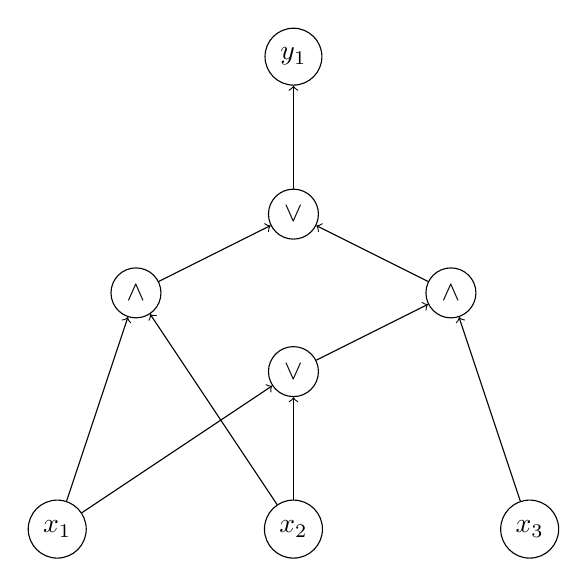
\begin{tikzpicture}
   \node[shape=circle,draw=black] (x1) at (0,0) {$x_1$};
    \node[shape=circle,draw=black] (x2) at (3,0) {$x_2$};
    \node[shape=circle,draw=black] (x3) at (6,0) {$x_3$};
    \node[shape=circle,draw=black] (t1) at (1, 3) {$\wedge$};
   \node[shape=circle,draw=black] (t2) at (3,2) {$\vee$};
    \node[shape=circle,draw=black] (t3) at (5,3) {$\wedge$};
    \node[shape=circle,draw=black] (t4) at (3,4) {$\vee$};
    \node[shape=circle,draw=black] (o) at (3,6) {$y_1$};

    \path [->] (x1) edge node[left] {} (t1);
    \path [->] (x1) edge node[left] {} (t2);
    \path [->] (x2) edge node[left] {} (t1);
    \path [->] (x2) edge node[left] {} (t2);
    \path [->] (x3) edge node[left] {} (t3);
    \path [->] (t2) edge node[left] {} (t3);
    \path [->] (t3) edge node[left] {} (t4);
    \path [->] (t1) edge node[left] {} (t4);
    \path [->] (t4) edge node[left] {} (o);
\end{tikzpicture}
 \\

	\caption{Булева схема, вычисляющая функцию $MAJ_3$}
\label{circuit}
\end{figure}


\subsection{Существующие решения}
Существует ряд алгоритмов для синтаксического анализа графов с использованием реляционной семантики запросов и контекстно-свободных грамматик~\cite{MatrixMult, HellingsCFPQ}, которые имеют низкую производительность на больших графах, так как их время работы в худшем случае порядка $O(n^5)$ для графа на $n$ вершинах. Известно, что существование алгоритма с субкубическим временем работы является открытой проблемой. В работе~\cite{MatrixMult} представлен алгоритм синтаксического анализа графов, использующий реляционную семантику запросов и КС-грамматики и вычисляющий матричное транзитивное замыкание с применением матричных операций, который позволяет использовать вычисления на графическом процессоре. Есть эффективный алгоритм, решающий данную задачу для Диковых и полу-Диковых языков на одном типе скобок, время работы которого составляет $O(n^{\omega}{\log{n}}^3)$, где $n$~--- число вершин в графе, а $n^{\omega}$~--- время умножения булевых матриц размером $n \times n$~\cite{Bradford}. Также в работе~\cite{ConjPath} представлен алгоритм, решающий задачу для конъюнктивных грамматик.

Параллельных алгоритмов, решающих задачу с использованием реляционной семантики на сегодняшний день не представлено. Очевидно, что задача не менее сложная, чем определение принадлежности строки $w$ контекстно-свободному яыку $L$. Для решения данной задачи имеются как булевы схемы, так и алгоритмы для других моделей параллельных вычислений~\cite{Brent, Ruzzo, Rytter}. Верхняя оценка для такой задачи~--- глубина схемы (параллельное время) $O(\log^2 n)$, где $n$~--- длина $w$.

Если рассматривать задачу как задачу пересечения регулярного языка с контекстно-свободным, то существует ряд булевых схем, решающих задачу проверки пустоты такого пересечения~\cite{Lohrey, Regularrealizability, Swernofsky2015OnTC}. Однако, рассматриваемая в данной работе задача состоит в перечислении такого пересечения, что не является задачей разрешимости как задача выше, поэтому требуется дополнительное исследование. Также есть оценки сложности для похожей задачи: фиксирована пара вершин $s$ и $t$ в графе, помеченном символами из языка $L$, и нужно ответить на вопрос, cуществует ли в графе путь из вершины $s$ в $t$, такой, что слово, полученное конкатенацией меток ребер этого пути, принадлежит языку $L$ (задача L-Reachability)~\cite{LReach}.
\subsection{Постановка задачи}
Как уже было сказано, алгоритмов, решающих задачу поиска путей с контекстно-свободными ограничениями эффективно, пусть даже на ограниченных подклассах графов, не представлено.
Представленные выше алгоритмы работают с графами произвольной
структуры. Если же исходный граф является ациклическим
(деревом), можно воспользоваться известными свойствами
ациклических графов, чтобы предоставить более
производительный алгоритм для решения задачи синтаксического
анализа для данной структуры графа. Например, многие эффективные алгоритмы синтаксического анализа \cite{Earley, Kasami, OkhotinParse, Valiant, Yonger} являются алгоритмами динамического программирования, где вычисления производятся отдельно для каждой подстроки. Корректность таких вычислений обеспечивается тем, что на символах строки задан порядок. В случае синтаксического анализа графа данные алгоритмы использовать затруднительно из-за нелинейного порядка на вершинах графа. По тем же причинам на таком входе нельзя использовать стратегию ``разделяй-и-властвуй``. Но известно, что на деревьях и ациклических графах порядок можно задать с помощью топологической сортировки. Так что одной из задач данной работы будет разработка и оценка алгоритма для синтаксического парсинга ациклических графов.
Так как параллельных алгоритмов для решения задачи не представлено, в данной работе будет построена булева схема, решающую задачу и оценены её параметры. Модель булевых схем удобна для оценки эффективности по сравнению с моделью PRAM, так как для нее существует большее количество классов cложности (${NC}^i$). Также интерес представляет зависимость эффективности булевой схемы от контекстно-свободной грамматики, для которой она построена, так как существуют КС-языки, распознавание которых с помощью схемы можно осуществить быстрее, чем в общем случае для произвольной контекстно-свободной грамматики~\cite{Dymond, Ibarra, LLComp}~--- будет ли такое преимущество существовать в случае синтаксического анализа графов?
\section{Синтаксический анализ ациклических графов}
В работе~\cite{OkhotinParse} предложен быстрый алгоритм синтаксического
анализа, основанный на матричных операциях и обобщённый для
булевых грамматик. С помощью булевых грамматик можно выразить
более широкий класс языков, а значит, формулировать более
сложные запросы к графам. В данном разделе будет предложено
расширение этого алгоритма для решения задачи синтаксического
анализа ациклических графов и показана его корректность.
\subsection{Аппроксимация решения}
Рассматриваемый ниже алгоритм основан на матричных операциях. Так как необходимо найти тройки $(A, i, j)$ для всех $A \in N$, результатом работы алгоритма на графе с $n$ вершинами будет матрица размером $n \times n$, в каждой из ячеек которой будут содержаться подмножества нетерминалов. На каждой итерации алгоритма, подмножества нетерминалов могут объединяться с помощью операции конъюнкции, если во входной грамматике существует соответствующее правило. Поэтому важно объединять только те нетерминалы, которые соответствуют одному и тому же уникальному пути между парой вершин графа. В случае, если входной ациклический граф является деревом, между любой парой вершин графа будет существовать всего один путь. Если же граф не является деревом, то между одной парой вершин может быть в худшем случае $2^{n-2}$ путей, поэтому хранить и обрабатывать данные для каждого пути отдельно неэффективно. Так как информацию о всех путях из вершины $i$ в вершину $j$ эффективно хранить в одной ячейке, то с помощью конъюнкции могут быть объединены нетерминалы, соответствующие разным путям из $i$ в $j$, но при этом будут объединены также нетерминалы, соответствующие одному и тому же пути, что и требуется для решения задачи. То же самое работает и для отрицаний в правиле: получив множества пар нетерминалов для одной пары вершин, необходимо проверить отсутствие в этом множестве определенных пар нетерминалов (согласно правилам грамматики). Так как неизвестно, какому конкретно пути соответствуют найденные нетерминалы, ответ будет неточным. Например, пусть в грамматике есть правило $A \to AB \wedge BC \wedge \neg DC$, а найденное множество пар нетерминалов для пары вершин $(i, j)$~--- $\{ AB, BC, DC\}$. Тогда, после применения упомянутого правила грамматики, ответ будет содержать утверждение $(i, j) \in R_A$. Но, полученное множество $\{ AB, BC, DC\}$ может выводить один и тот же уникальный путь между вершинами $i$ и $j$, тогда из-за отрицания $DC$, не будет существовать пути из вершины $i$ в вершину $j$, образующего строку, выводимую из нетерминала $A$. Алгоритм рассматривает все возможные сочетания пар нетерминалов, в результате могут появится лишние вершины $(i,j)$, если в графе не существует пути из $i$ в $j$, соответствующего рассмотренным подмножествам пар и правилу для них.

Поэтому приведенный ниже алгоритм будет вычислять аппроксимацию сверху для отношений $R_A$ (надмножество необходимого множества).
\subsection {Описание алгоритма}
Пусть $n$ - число вершин в графе $D$, вершины графа пронумерованы. $G = (N, \Sigma, S, R)$~--- булева грамматика в нормальной форме.

Алгоритм использует следующие структуры данных:
\begin{enumerate}
\item Таблица парсинга $T$ размером $n \times n$, представляющая собой верхнетреугольную матрицу, где для каждый элемент $T_{i, j}$ является множеством нетерминалов.

Пусть $X \in {(2^N)}^{m \times l}$ и $Y \in {(2^N)}^{l \times n}$ – матрицы подмножеств множества нетерминалов $N$, а $m, l, n$ – натуральные числа, большие единицы. Тогда зададим произведение матриц $X \times Y$ как матрицу $Z \in {(2^N)}^{m \times n}$, такую, что каждый её элемент $Z_{i, j}$ вычисляется по следующей формуле:
\begin{equation}\label{eq:mult}
Z_{i,j} = \bigcup_{k=1}^{l}X_{i,k} \times Y_{k, j}
\end{equation}
\item Таблица $P$, элементы $P_{i,j}$ которой принадлежат множеству пар нетерминалов $N \times N$.
\end{enumerate}

Используя значения $P_{i,j}$, можно получить набор нетерминалов для таблицы $T$~--- объединить пары нетерминалов в конъюнкты согласно правилам грамматики.
\begin{equation}
T_{i,j} = f(P_{i,j}),
\end{equation}
где $f: 2^{N \times N} \to 2^N$ для булевых грамматик определяется по формуле
\begin{equation*}
\begin{aligned}
f(P) = \bigcup_{k=1}^{2^{|P|}} \{A| \exists A \to B_1C_1 \wedge ... \wedge B_mC_m \wedge \neg D_1E_1 \wedge ... \wedge D_m'E_m' \\
\in R: (B_t, C_t) \in P^k, (D_t, E_t) \not\in P^k \forall t\},
\end{aligned}
\end{equation*}
где $P^k$~--- подмножество множества $P$. Функция $f$ обеспечивает аппроксимацию сверху для операции отрицания: благодаря тому, что рассмотриваются все подмножества нетерминалов, в результате не будут отсечены нужные отношения, например $P_{i,j} = \{AB, BC, CD\}$, и в грамматике есть правило $S \to AB \wedge BC \wedge \neg CD$. При этом, если в графе $AB \wedge BC$ соответствует одному пути из $i$ в $j$, а $CD$~--- другому, то $(i,j) \in R_S$. В итоге для $P^k = \{AB, BC\}$ функция $f$ вернёт $S$.

В алгоритме Охотина элементы матрицы $P$ рассчитываются
группами с помощью выше определенного произведения
подматриц (3) из таблицы $T$, дающих аналогичный результат с
поэлементным умножением. Схема расположения подматриц
представлена на рис.~\ref{submatrices1},~\ref{submatrices2}.

Алгоритм состоит из двух рекурсивных процедур:
\begin{enumerate}
\item $compute(l, m)$~--- рассчитывает значения $T_{i,j}$ для любых $l \le i < j < m$.
\item $complete(l, m, l', m')$~--- определена для $l \le m < l' \le m'$ при $m - l = m' - l'$ и $m - l$ без потери общности являющимися степенью двойки.

Четыре входных параметра процедуры обозначают координаты
подматрицы матрицы $T$, содержащей все элементы $T_{i,j}$, где $l \le i < j < m$ и $l' \le j < m'$. Они обозначают пути в графе, номер начала которых лежит между $l$ и $m$, а конец между $l'$ и $m'$. Так как ранее уже посчитаны $T_{i,j}$ для $l \le i < j < m$ и $l' \le i < j < m'$, а также $P_{i,j}$ для $l \le i < m$ и $l' \le j < m'$, процедура $complete(l, m, l', m')$ получает значения $T_{i,j}$ для $l \le i < m$ и $l' \le j < m'$.
\end{enumerate}
\begin{figure}
\centering
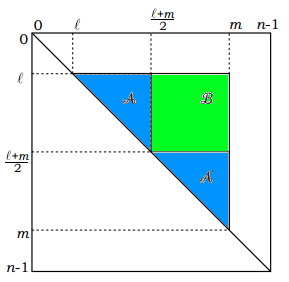
\includegraphics[width=0.45\textwidth]{Shemetova/subm1.png}
\caption{Расположение подматриц матрицы $T$ для вычисления произведений}
\label{submatrices1}
\end{figure}
\begin{figure}
\centering
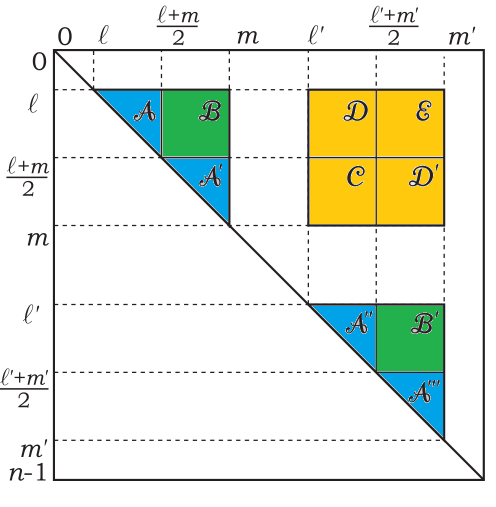
\includegraphics[width=0.45\textwidth]{Shemetova/sub1.jpg}
\caption{Расположение подматриц матрицы $T$ для вычисления произведений}
\label{submatrices2}
\end{figure}

Так как основная структура данных, с которой работает алгоритм,
является верхнетреугольными матрицами, то тогда должен быть
задан линейный порядок на вершинах графа $D$, такой, что любое
ребро ведет от вершины с меньшим номером к вершине с
большим номером. Если $D$ является ациклическим графом, то
данного свойства легко добиться с помощью топологической
сортировки графа. Например, алгоритм Тарьяна~\cite{Tarjan} позволяет
осуществлять топологическую сортировку за линейное от
количества вершин графа время $O(n)$.

Полный псевдокод алгоритма приведен в листинге \ref{DAGalg}.
\begin{algorithm}
\caption{Алгоритм для синтаксического анализа ациклических графов}\label{DAGalg}
 \hspace*{\algorithmicindent} \textbf{Вход:} $D = (V, E)$~--- ациклический граф с пронумерованными вершинами, \\$G$~--- булева грамматика.\\
 \hspace*{\algorithmicindent} \textbf{Выход:} матрица $T$
\begin{algorithmic}[1]
\State $n \gets |V|$
\State $D \gets TopologicalSorting(D)$
\State $T \gets T[0][0], T[0][1], ... , T[n] [n]$
\State $P \gets P[0][0], P[0][1], ... , P[n] [n]$
\For{$(i, j, a) \in E$}
\State $T_{i,j} \gets \{A \mid A \to a \in R\}$
\EndFor
\State $compute(0, n-1)$
\Procedure{compute}{$l, m$}
\If {$m-1 \ge 4$}
\State $compute(l, \frac{l+m}{2})$
\State $compute(\frac{l+m}{2},m)$
\EndIf
\State $complete(l, \frac{l+m}{2}, \frac{l+m}{2}, m)$
\EndProcedure
\Procedure{complete}{$l, m, l', m'$}
\If {$(l, m, a) \in E$ and $m < l'$}
\State $T_{l,l'} \gets f(P_{l,l'})$
\ElsIf {$m-1 >1$}
\State $B \gets (l, \frac{l+m}{2}, \frac{l'+m'}{2}, m')$
\State $B' \gets (\frac{l+m}{2}, m, l', \frac{l'+m'}{2})$
\State $C \gets (\frac{l+m}{2}, m, l', \frac{l'+m'}{2})$
\State $D \gets (l, \frac{l+m}{2}, l', \frac{l'+m'}{2})$
\State $D' \gets (\frac{l+m}{2}, m, \frac{l'+m'}{2}, m')$
\State $E \gets (l, \frac{l+m}{2}, \frac{l'+m'}{2}, m')$
\State $complete(C)$
\State $P_D \gets P_D \cup (T_B \times T_C)$
\State $complete(D)$
\State $P_{D'} \gets P_{D'} \cup (T_C \times T_{B'})$
\State $complete(D')$
\State $P_{E} \gets P_{E} \cup (T_B \times T_{D'})$
\State $P_{E} \gets P_{E} \cup (T_D \times T_{B'})$
\State $complete(E)$
\EndIf

\EndProcedure

\end{algorithmic}
\end{algorithm}

\subsection {Корректность алгоритма}
Как было сказано выше, алгоритм вычисляет приближенное решение, в итоге будут получены надмножества всех искомых булевых отношений для пар вершин. Результат работы алгоритма будет содержаться в ячейках матрицы $T$.
Корректность алгоритма следует из выполнимости следующих утверждений.
\begin{theoremrus} (Корректность алгоритма для синтаксического
анализа ациклических графов). Пусть даны помеченный
ациклический граф $D$ и булева грамматика $G = (\Sigma, N, R)$.
Тогда для любых вершин $i, j$ и для любого нетерминала $A \in N$, если
$(i, j) \in R_A$, то $A \in T_{i,j}$.
\end{theoremrus}
\textit{Доказательство.} Рассмотрим такие вершины $i,j$, что $(i, j) \in R_A$ и существует $i \pi j$, такой, что $l(\pi) \in L(G_A)$ (т.е. существует дерево разбора для строки $l(\pi)$ и грамматики $G$ с корнем в нетерминале $A$). Докажем индукцией по высоте дерева разбора строки $l(\pi)$, что $A \in T_{i,j}$.

\textit{База индукции}. Если $(i, j)$~--- ребро графа (высота дерева разбора равна 1), то алгоритм корректен, исходя из инициализации
матрицы $T$ (строки 5-6 листинга \ref{DAGalg}).

\textit{Индукционный переход}. Предположим, утверждение верно для
всех деревьев разбора высотой $n$. Докажем, что теорема верна для
деревьев разбора высотой $n+1$. Рассмотрим дерево разбора для $l(\pi)$ высотой $n+1$. Так как
грамматика в нормальной форме, то у данного дерева будут
поддеревья, выводящие подстроки $l(\pi)$ (возможно
пересекающиеся). По свойству топологической сортировки для
всех индексов $k,l$ этих подстрок (начала и конца соответствующих
путей) выполняется неравенство $i \le k < m \le j$.

Вызов $compute(i, j)$ посчитает $T_{i,j}$ для всех $i \le k < l < j$. По индукционному предположению, для всех подпутей
$k \pi' m$ пути $i \pi j$ и нетерминалов $A \in T_{k,m}$ верно, что если $(k, m) \in R_A$, то $A \in T_{k,m}$.

$T_{i,j}$
вычисляется как $f(P_{i,j})$. $P_{i,j}$ по алгоритму \ref{DAGalg} может быть получено
тремя способами, в зависимости от положения подматрицы, в
которой оно задано. Пусть $P_{i,j}$~--- ячейка матрицы $P_Z$. В любом из
случаев $P_Z$ вычисляется как $P_Z \cup (T_X \times T_Y)$. По определению
произведения $T_X \times T_Y$ (\ref{eq:mult}), для каждого пути $i, j$ будут получены все
произведения нетерминалов из конъюнктов, выводящих все
подстроки $l(\pi)$, такие, что путь $i \pi j$ разбит на две части вершиной
$k$, такой что $i < k < j$. По индукционному предположению, т.е. если $(i,k) \in R_B$, то $B \in T_{i,k}$ и если $(k,l) \in R_C$, то $C \in T_{k, j}$. Тогда
произведение матриц $T_X \times T_Y$ даст все возможные пары нетерминалов $\{(BC)\} \in P_{i,j}$ для всех подстрок. После применения функции $f$ (подбора соответствующго правила грамматики), $T_{i,j}$ будет содержать нетерминалы, полученные после применения правил. Тогда, исходя из правил грамматики, получим, что если $(i,j) \in R_A$, то $A \in T_{i, j}$ (объединяем существующие поддеревья для подстрок в одно дерево). А это значит, что утверждение верно для дерева разбора высотой $n + 1$.

Время работы алгоритма аналогично времени работы алгоритма
Охотина~\cite{OkhotinParse} и составляет $O(|G|BMM(n) \log n)$, где $|G|$~--- размер
входной булевой грамматики, $n$~--- число вершин в графе $D$,
$BMM(n)$ – время умножения булевых матриц размера $n \times n$.

\section {Булева схема для синтаксического анализа графов}
Булева схема будет построена основе алгоритма Брента-Гольдшлягера-Риттера~\cite{Brent}. Идея алгоритма соcтоит в построении системы логического вывода и доказательства утверждений вида $A(i, j)$, где $A$~--- нетерминал, а $i, j$~--- начало и конец пути в $D$ cоответственно. В предложенной ниже системе вывода также будут существовать условные утверждения вида ``если $D(k, l)$, то $A(i, k::l, j)$``, где $i::j$ обозначает \textit{дырку}, оставленную в пути из вершины $i$ в вершину $j$ cо свойством $A$ для подотрезка этого пути из вершины $k$ в вершину $l$ со свойством $D$. Дерево разбора для $A(i, j)$ и дерево разбора $A(i, j)$ с дыркой $D(k, l)$ представлены на рис.~\ref{hole}.

\subsection {Система вывода}
Дан ориентированный граф $D$ с пронумерованными вершинами и контекстно-свободная грамматика в нормальной форме Хомского.

Тогда используется система вывода со следующими правилами:
\begin{table}[ht]
  \centering
  \begin{tabular}[t]{l l}
   $\frac{}{A(i , j)}$ &(метка ребра $i \xrightarrow a j$ , если $A \rightarrow a \in P$,
   \\ &   $i , j \in E$ и помечено символом $a \in \Sigma$)\\
    & \\
   $\frac{B(i , j)}{\frac{A}{C}(i , j :: z)}$  & (создание дырки справа, 
    \\ & если  $A \rightarrow BC \in P$ и $z \in V$) \\
   & \\
   $\frac{C(j  , z)}{\frac{A}{B}(i :: j  , z)}$  & (создание дырки слева, 
   \\ & если  $A \rightarrow BC \in P$ и $i \in V$) \\
   &\\
   $\frac{\frac{A}{D}(i , j :: w , z), D(j , w)}{A(i  , z)}$  & (затыкание дырки) \\
   &\\
   $\frac{\frac{A}{E}(i , j :: w  , z), \frac{E}{D}( j , u :: v , w)}{\frac{A}{D}(i, u :: v , z)}$  & (соединение условных утверждений) \\
\end{tabular}
\end{table}
\subsection {Оценка глубины рекурсии}
\begin{figure}[!]
\centering
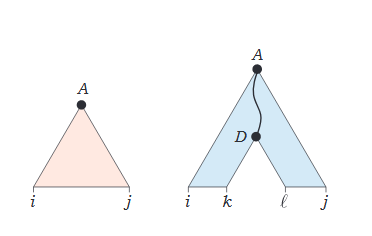
\includegraphics[width=0.5\textwidth]{Shemetova/trees.png}
\caption{Дерево разбора для $A(i, j)$ (слева) и дерево разбора $A(i, j)$ с дыркой $D(k, l)$ (справа)}
\label{hole}
\end{figure}
\begin{lemmarus}\label{TreeLem}
Пусть $G$~--- грамматика в нормальной форме Хомского. Тогда всякое дерево разбора с $\zeta$ листьями содержит вершину (будем называть ее промежуточной), в чьём поддереве более чем $\frac{1}{3}\zeta$ листьев, и менее $\frac{2}{3}\zeta$ листьев.
\end{lemmarus}
\textit{Доказательство.} Путь строится сверху, каждый раз выбирается наибольшее поддерево. Так как ветвление двоичное, искомая вершина найдется (рис.~\ref{e}). Данная лемма иллюстрирует тот факт, что дерево разбора можно разбить на три меньших поддерева.


\begin{lemmarus}\label{Depthlem}
Пусть $\zeta$~--- длина пути из вершины $i$ в $j$. Тогда в системе вывода всякое утверждение $\frac{A}{D}(i , u :: v , j)$ или $A(i , j)$ имеет доказательство высоты не более чем $4\log_{3/2}\zeta$.
\end{lemmarus}
\textit{Доказательство.} Индукция по $\zeta$.

Если t~--- путь в графе, то дерево разбора для этого пути будет содержать $\zeta$ листьев (каждое ребро помечено терминальным символом). По Лемме \ref{TreeLem} для дерева разбора $A(i, j)$ найдется промежуточная вершина, назовём её $E$, а её детей $B$ и $C$ ($E \rightarrow BC \in P$). Тогда вывод $A(i , j)$ можно записать следующим образом:
\begin{prooftree}
\AxiomC{$B(u, l)$}
\AxiomC{$C(l, v)$}
\BinaryInfC{$E(u, v)$}
\AxiomC{$\frac{A}{E}(i , u :: v , j)$}
\BinaryInfC{$A (i, j)$}
\end{prooftree}

По свойству промежуточной вершины, количество листьев в поддеревьях $\frac{A}{E}(i , u :: v , j)$, $B(u, l)$, $C(l, v)$ не превышает $\frac{2}{3}\zeta$. По предположению индукции, для них есть доказательства логарифмической высоты.

Для $\frac{A}{D}(i , u :: v , j)$ рассмотрим два случая: 1) дерево промежуточной вершины включает в себя дырку и 2) дерево промежуточной вершины содержит только листья, относящиеся к пути $i \rightarrow u$ (или $v \rightarrow j$).

\textit{Первый случай}. Пусть промежуточная вершина помечена символом $E$. Так как поддерево этой вершины содержит дырку, то оно разбивает путь $i \rightarrow u$ на два пути вида $i \rightarrow k$ и $k \rightarrow u$, а путь $v \rightarrow j$ на $v \rightarrow l$ и $l \rightarrow j$.
Тогда вывод $\frac{A}{E}(i , u :: v , j)$ можно записать так:
\begin{prooftree}
\AxiomC{$\frac{A}{E}(i , k :: l , j)$}
\AxiomC{$\frac{A}{D}(k , u :: v , l)$}
\BinaryInfC{ $\frac{A}{E}(i , u :: v , j)$}
\end{prooftree}

\textit{Второй случай}. Пусть дерево промежуточной вершины содержит только листья, относящиеся к пути $i \rightarrow u$. Рассмотрим наибольшее поддерево, включающее данное, и содержащее только листья, относящиеся к пути $i \rightarrow u$. Пусть это поддерево помечено нетерминалом $B$ и выводит путь $k \rightarrow l$, являющийся подпутем $i \rightarrow u$. Пусть $E$ - родитель $B$, а $C$ - второй потомок $E$ ($E \rightarrow BC \in P$). Тогда $С$ будет разбивать путь $v \rightarrow j$ на $v \rightarrow m$ и $m \rightarrow j$. Тогда вывод для $\frac{A}{E}(i , u :: v , j)$ выглядит так:
\begin{prooftree}

\AxiomC{$\frac{A}{E}(i , k :: m , j)$}
\AxiomC{$B(k, l)$}
\UnaryInfC{$\frac{E}{C}(k , l :: m)$}
\AxiomC{$\frac{C}{D}(l , u :: v , m)$}
\BinaryInfC{$\frac{E}{D}(k , u ::v , m)$}
\BinaryInfC{ $\frac{A}{D}(i , u :: v , j)$}
\end{prooftree}
Так как $B(k, l)$ содержит не менее чем $\frac{1}{3}\zeta$ листьев, то утверждения $\frac{A}{E}(i , k :: m , j)$ и $\frac{C}{D}(l , u :: v , m)$ содержат менее $\frac{2}{3}\zeta$ листьев каждое, поэтому по предположению индукции они имеют доказательство логарифмической высоты. Для утверждений вида $B(k, l)$ уже доказано существование доказательства логарифмической высоты. Получаем, что дерево $\frac{A}{D}(i , u :: v , j)$ с $\zeta$ листьями выводится за 4 шага из поддеревьев не более чем с $\frac{2}{3}\zeta$ листьями.
\begin{lemmarus}\label{Depthzeta}
Пусть $\zeta$~--- максимальная длина пути, являющегося ответом на задачу поиска путей с контекстно-свободными ограничениями. Тогда глубина булевой схемы для решения данной задачи составляет $O(\log^2 \zeta)$.
\end{lemmarus}
\begin{figure}[!]
\centering
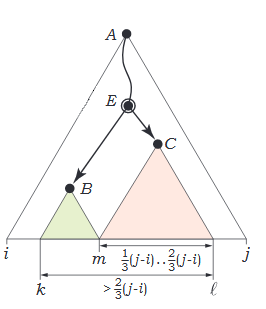
\includegraphics[width=0.35\textwidth]{Shemetova/e.png}
\caption{Промежуточная вершина $E$ и два её поддерева}
\label{e}
\end{figure}
\textit{Доказательство.} На стеке на каждом уровне рекурсии осуществляется не более $\log \zeta$ операций, глубина рекурсии по Лемме \ref{Depthlem}~--- $O(\log \zeta)$.
\begin{corollaryrus} Пусть дан ациклический граф $D$ c $|V|=n$ и контекстно-свободная грамматика $G$. Тогда глубина схемы для синтаксического анализа ациклического графа~--- $O(\log^2 n)$.
\end{corollaryrus}
\textit{Доказательство.} Произведем топологическую сортировку графа $D$. Так как максимальная длина пути в таком графе не превысит $n$, то $\zeta$ также меньше $n$. Отсюда получаем искомую оценку.
\subsection {Описание схемы}
\textbf{Вход:} Элементы вида $(a, i, j)$, где $i, j$~--- смежные вершины графа, $a \in \Sigma$~--- помечено ли ребро из $i$ в $j$ nерминалом $a$. Количество входных элементов~--- $|\Sigma| \cdot n^2$

\textbf{Элементы:}
\begin{itemize}
  \item Для всех вершин $i, j$, где $1 \leq i, j \leq n$, есть элемент $x_{A, i, j}$, в котором вычисляется значение $A(i, j)$, то есть принадлежит ли слово, составленное из меток пути $i \rightarrow ... \rightarrow j$ языку $L_G(A).$
  \item Элемент $y_{A,i,j,D,k,l}$, где $A, D \in N, 1 \leq i, j, k, l \leq n $. Этот элемент определяет, существует ли дерево разбора пути $i \rightarrow ... \rightarrow j$ из $A$, с дыркой вместо поддерева $k \rightarrow ... \rightarrow l$ из $D$, так что в нём вычисляется значение 1 тогда и только тогда, когда верно условное утверждение $\frac{A}{D}(i \rightarrow... \rightarrow k :: l \rightarrow... \rightarrow j )$.
\end{itemize}
\textbf{Выход:} Элементы вида $(A, i, j)$~--- cуществует ли поддерево разбора с нетерминалом $A$ в корне для строки, полученной конкатенацией терминальных символов ребер пути из вершины $i$ в $j$. Таких элементов $|N| \cdot n^2$. 

Данные вычисления можно адаптировать для модели параллельных вычислений SIMDAG.

\subsection {Описание алгоритма для модели SIMDAG}
Параллельный алгоритм для решения задачи поиска путей с контекстно-свободными ограничениями для модели параллельных вычислений SIMDAG аналогичен модифицированному алгоритму Брента-Гольдшлягера-Риттера~\cite{Brent}. Модификации включают в себя:
\begin{itemize}
  \item снятие ограничения на порядок индексов (например, требование для $A(i, j)$ вида $i \leq j$)~--- данные модификации носят формальный характер, так как не влияют на порядок и состав вычислений в оригинальном алгоритме
  \item добавление выходных элементов~--- для каждого элемента $x_{A, i, j}$ добавлен аналогичный выходной, так как для решения задачи контекстно свободной-достижимости необходимо ответить на вопрос о достижимости всех возможных видов путей в графе
\item увеличение количества итераций до $4\log_{3/2}t$, где $t$~--- максимальная длина строки, являющейся ответом на задачу.
\end{itemize}
Ниже приведен псевдокод модифицированного алгоритма:
\begin{algorithm}[h!]
\caption{Алгоритм Брента-Гольдшлягера-Риттера для решения задачи поиска путей с контекстно-свободными ограничениями}\label{alg:BGR}
\begin{algorithmic}[1]
\State $\textit{$P(x_{A, i, j})$} \gets \textit{$P[0], P[1], ... , P[Nn^2 - 1]$}$
\State $\textit{$Q(y_{A,i,j,D,k,l})$} \gets \textit{$Q[0][0], Q[0][1], ... , Q[Nn^2 - 1] [Nn^2 - 1]$}$
\If {$\textit{$(i , a, j) \in E$} \text{ and } \textit{$A \rightarrow a $}$}
\State $P(x_{A, i, j}) \gets \text{true}$
\EndIf
\For{$\textit{t = 1} \text{ to } \textit{$4\log_{3/2}t$}$}
\State $\textit{$U(y_{A,i,j,D,k,l})$} \gets \textit{$Q(y_{A,i,j,D,k,l})$}$
\If {$(C \rightarrow DE) \in P$ and (($Q(y_{D,p,q,B,x,y})$ and $P(x_{E, q, r})$)
\\ \hspace*{5em} or ($(P(x_{D, p, q})$ and $Q(y_{E,q,r,B,x,y})$))}
\State $U(y_{C,p,r,B,x,y}) \gets \text{true}$
\EndIf
\If {$U(y_{A,i,j,C,p,r})$ and $U(y_{C,p,r,B,x,y})$}
\State $Q(y_{A,i,j,B,x,y}) \gets \text{true}$
\EndIf
\State $V(x_{A, i, j}) \gets P(x_{A, i, j})$
\If {$(C \rightarrow DE) \in P$ and $P(x_{D, p, q})$ and $P(x_{E, q, r})$}
\State $V(x_{C, p, r}) \gets \text{true}$
\EndIf
\If {$Q(y_{A,i,j,C,p,r})$ and $V(x_{C, p, r})$}
\State $P(x_{C, p, r}) \gets \text{true}$
\EndIf
\EndFor
\end{algorithmic}
\end{algorithm}

\textbf {Оценка времени работы и количества процессоров}

Операцией, которая задействует наибольшее количество элементов в исходном алгоритме, является операция соединения условных утверждений: \textit{$U(y_{A,i,j,C,p,r})$} \text{$ \land $} \textit{$U(y_{C,p,r,B,x,y})$}. Она требует $N^2n^4 \times Nn^2 = N^3n^6$ элементов. В модифицированной версии общее количество элементов не меняется, за исключением добавления дополнительных выходных элементов, число которых $Nn^2$. Поэтому количество элементов в схеме $O(n^6)$, если считать число нетерминалов константой.

Из Леммы~\ref{Depthzeta} и построения алгоритма следует, что его время работы равно $O(\log^2t)$ на unit-cost SIMDAG и $O(\log t)$ на log-cost SIMDAG.

\section {Оценка глубины схемы для различных классов контекстно-свободных грамматик}В частях 2.3~--- 2.5 будут анализироваться деревья разбора для грамматики в разных нормальных формах: нормальная форма Хомского (2.3) и квадратичная нормальная форма Грейбах (2.5). Перевод в НФХ увеличивает высоту дерева в константу раз, то же самое увеличение дает перевод в форму Грейбах~\cite{Kelemenova}. Таким образом, конкретная форма грамматики асимптотически не повлияет на анализируемые параметры.
\subsection{Минимальная строка}
В предыдущем разделе было показано, что высота схемы зависит от минимальной длины строки $\zeta$, являющейся ответом на задачу. Определим её формально следующим образом.

Пусть дана контекстно-свободная грамматика $G$, где $A \in N$ и помеченный ориентированный граф $D$, где $m, n \in V$, такие что $\mathzapf{L} = \mathzapf{L}(G; A) \cap \mathzapf{L}(D; m, n)$. Тогда $\zeta = \max\limits_{\forall(m,n)}\min ||\mathzapf{L}||$.

Например, для графа на рис.~\ref{graph} и контекстно-свободной грамматики $G = (\{S\}, \{a, b\},\\ \{S \rightarrow aSb,
S \rightarrow \varepsilon\})$ $\zeta = 12$ (путь из вершины с номером 3 в вершину 3, соответствующая последовательность~--- "aaaaaabbbbbb" ).

В работе~\cite{HellingsCFPQ} даны следующие верхняя и нижняя оценки на $\zeta$:
\begin{itemize}
\item Нижняя оценка: $\zeta \ge \frac{2^{|N|}n^2}{64} $.
\item Верхняя оценка: $\zeta \le 2^{|N|n^2}$,
\end{itemize}
где $n$~--- число вершин в графе, $|N|$~--- число нетерминалов в контекстно-свободной грамматике.
\begin{figure}
\centering

\begin{tikzpicture}[shorten >=1pt,node distance=2cm,on grid,auto]
   \node[state] (q_1) {$1$};
   \node[state] (q_2) [above right=of q_1] {$2$};
   \node[state] (q_3) [right=of q_2] {$3$};
   \node[state] (q_4) [right=of q_3] {$4$};
    \path[->]
    (q_1) edge  node {a} (q_2)
    (q_2) edge  node {a} (q_3)
    (q_3) edge  node {a} (q_1)
    (q_3) edge[bend left, above]  node {b} (q_4)
    (q_4) edge[bend left, below]  node {b} (q_3);
\end{tikzpicture}
\\
	\caption{Помеченный ориентированный граф}
\label{graph}
\end{figure}
\subsection{Рациональный индекс}
В связи с тем, что для схемы фиксирована грамматика, а граф подаётся на вход, интересно рассмотреть взаимосвязь $\zeta$ и числа вершин в графе при фиксированной кс-грамматике.
Такую связь описывает специальный показатель сложности контекстно-свободных языков~--- \textit{рациональный индекс}. Ниже дано его определение.

Пусть фиксирован некоторый контекстно-свободный язык $L$. Пусть $Rat_n$~--- семейство регулярных языков, распознаваемых конечным автоматом с не более чем $n$ состояниями. Тогда \textit{рациональный индекс} $p_L(n)$ языка $L$ определяется как функция вида $\mathbb{N} \rightarrow \mathbb{N}$:
\begin{equation}
p_L(n) = \max\limits_{K \in Rat_n | K  \cap L \neq \emptyset} \min\limits_{w \in K  \cap L } |w|
\end{equation}
Нетрудно заметить, что рациональный индекс описывает поведение величины $\zeta$ для фиксированного кс-языка в зависимости от увеличения количества вершин в графе (действительно, каждому графу можно однозначно сопоставить конечный автомат, а конечному автомату~--- регулярный язык). Поэтому, зная величину рационального индекса, можно получить верхнюю и нижнюю оценки высоты схемы для распознавания данного языка.

На текущий момент известны верхние оценки для рационального индекса следующих языков:
\begin{itemize}
	\item Язык Дика на одном типе скобок $D_1'^* = (\{S\}, \{a, b\}, \{S \rightarrow aSbS, S \rightarrow \varepsilon\})$~--- $p_L(n) = O(n^2)$~\cite{Dyck1}.
	\item Языки Грейбах $H$~--- $p_L(n) = \Theta(n^\lambda)$, где $\lambda$~--- алгебраическое число больше 1~\cite{GreibRat}.
	\item Произвольный контекстно-свободный язык~--- $p_L(n) = \Theta(2^ {\frac{n^2}{\ln n}})$~\cite{CFRat}.
\end{itemize}
Исходя из Леммы~\ref{Depthzeta}, получаем:
\begin{corollaryrus} Пусть дан граф $D$ c $|V|=n$ и контекстно-свободная грамматика $G$. Тогда в общем случае глубина схемы для синтаксического анализа графа будет полиномиальной от входа $t = \Sigma n^2$~--- $O(t^2)$ для константного $\Sigma$, в случае если $L(G) = D_1'^*$ или $L(G) = H$ полилогарифмической~--- $O(\log^2 n)$.
\end{corollaryrus}

\subsection{Оценка глубины схемы для линейных грамматик}
\begin{figure}[h!]
\centering

\begin{tikzpicture}
\node{S}
 child {node {a}}
 child {node {$A$}
      child {node {b}}
      child { node {$B$}
        child { node {$C$}
                     child {node {d}}
                     child { node {$...$}} }
        child { node {$c$}} }
     };
\end{tikzpicture}
 \\
	\caption{Дерево разбора для линейной грамматики в нормальной форме Хомского}
\label{Linw}
\end{figure}
\textit{Линейная грамматика}~--- контекстно-свободная грамматика, которая имеет не более одного нетерминала в правой части каждого правила.

Пусть $T$~--- множество терминалов. Линейная грамматика $G = (N, T, \Sigma, P)$ находится в \textit{нормальной форме Хомского} тогда, когда любое её правило имеет одну из следующих форм: $A \rightarrow aB$, $A \rightarrow Ba$, $A \rightarrow a$, где $B \in N$ и $a \in T$.
\begin{lemmarus}
\label{Heightlem} Пусть дана контекстно-свободная грамматика $G$, где $A \in N$ и помеченный ориентированный граф $D$, где $m, n \in V$, такие что $\mathzapf{L} = \mathzapf{L}(G; A) \cap \mathzapf{L}(D; m, n)$. Пусть $l = \min ||\mathzapf{L}||$. Тогда высота дерева разбора строки $l$ не превышает $|N|V^2$ для любых $m, n$.
\end{lemmarus}
\textit{Доказательство.} Пусть у дерева разбора $l$ высота больше, чем $|N|V^2$. Так как $l$ минимальная, то все её подстроки минимальны (в противном случае мы могли бы заменить большую на меньшую). Уникальных троек вида $(A, i, j)$ всего $|N|V^2$, тогда по принципу Дирихле в дереве разбора для $l$ будет как минимум одно поддерево $T$, соответствующее какой-либо из троек и содержащее поддерево $T'$, соответствующее такой же тройке, но выводящее строку длиной меньше. Тогда заменив $T$ на $T'$ получим строку длиной меньше, чем $l$. Но по условию $l$~--- минимальная, получаем противоречие.
\begin{theoremrus}
Глубина схемы синтаксического разбора графа $D$ на $n$ вершинах для случая линейной грамматики $G$ равна $O(\log^2 n)$.
\end{theoremrus}

\textit{Доказательство.} Оценим величину показателя $\zeta$ для линейной грамматики. Рассмотрим дерево разбора для строки длины $\zeta$, по Лемме~\ref{Heightlem} его высота не превосходит $|N|n^2$, оно изображено на рис.~\ref{Linw}. Будем спускаться от корня дерева вниз, считая листья. Так как линейная грамматика в нормальной форме Хомского, то спуск на один уровень добавит только один лист к общему количеству листьев. На самом последнем уровне по правилу $A \rightarrow a$ дерево закончится. Отсюда получаем, что количество листьев равно высоте дерева, а именно не превосходит $|N|n^2$. Тогда $\zeta \le |N|n^2$, а значит высота схемы в случае линейной грамматики равна $\log^2(|N|n^2) = O(\log^2 n)$ при константном числе нетерминалов.
\subsection{Оценка глубины схемы для input-driven грамматик}
\textit{Input-driven грамматика} $G = ( \Sigma, N, S, P)$ определена следующим образом~\cite{IDGrammar}:
\begin{itemize}
	\item $\Sigma = \Sigma_{+1} \cup \Sigma_0 \cup \Sigma_{-1}$~--- алфавит, разделенный на три непересекающихся класса.
	\item $N$~--- множество нетерминальных символов.
         \item $S$~--- стартовый нетерминал, $S \in N$.
	\item $P$~--- набор правил, каждое из которых находится в следующей форме: либо $A \rightarrow <B>C$, либо $A \rightarrow aC$, либо $A \rightarrow \varepsilon$, где $A, B, C \in N$, $< \in \Sigma_{+1}$, $> \in \Sigma_{-1}$, $a \in \Sigma$.
\end{itemize}
Примером input-driven языка является язык $L = \{a^nb^n | n \ge 2\} \cup \{a^nc^n | n \ge 2\}$.

Input-driven язык и распознаются специальным видом автоматов~--- \textit{автоматами с магазинной памятью, управляемыми входом (IDPDA)}. Дадим формальное определение таких автоматов~\cite{OkhotinIDPDA}:

\textit{Детерминированный автомат с магазинной памятью, управляемый входом (DIDPDA)} определён как семёрка $A = (\Sigma, Q, \Gamma, q_0, \bot, [\delta_a], F)$, где:
\begin{itemize}
	\item $Q$~--- конечное множество состояний автомата с начальным состоянием $q_0 \in Q$ и множеством конечных состояний $F \subseteq Q$.
	\item $\Gamma$~--- конечный стековый алфавит, символ $\bot \not\in \Gamma$ означает пустой стек.
         \item Функция перехода для открывающей скобки $< \in \Sigma_{+1}$~--- частичная функция $\delta_<: Q \rightarrow Q \times \Gamma$, которая для текущего состояний показывает следующее состояние и символ, добавляемый в стек.
         \item Функция перехода для закрывающей скобки $> \in \Sigma_{-1}$~--- частичная функция $\delta_>: Q \times (\Gamma \cup \{ \bot \}) \rightarrow Q$, которая для текущего состояний показывает следующее состояние, подразумевая, что указанный символ вынут из стека или стек пустой.
	\item Для нейтрального символа $c \in \Sigma_0$, изменение состояние описывается частичной функцией $\delta_c: Q \rightarrow Q$.
\end{itemize}
\textit{Koнфигурация} $A$~--- тройка $(q, w, x)$, где $q \in Q$~--- состояние, $w \in \Sigma^*$~--- оставшийся вход и $x \in \Gamma^*$~--- содержимое стека. Начальная конфигурация при входной строке $w_0 \in \Sigma^*$--- $(q_0, w_0, \varepsilon)$. Для каждой конфигурации с как минимум одним оставшимся символом следующая конфигурация определяется единственным образом согласно следующим правилам:
\begin{itemize}
         \item Для каждой открывающей скобки < $\in \Sigma_{+1}$ $(q, <w, x) \vdash_A (q', w, \gamma x)$, где $\delta_<(q) = (q', \gamma)$.
         \item Для каждой открывающей скобки > $\in \Sigma_{-1}$ $(q, >w,\gamma x) \vdash_A (\delta >(q, \gamma), w, x)$, а в случае пустоты стека $(q, >w, \varepsilon) \vdash_A (\delta_>(q, \bot), w, \varepsilon)$.
	\item Для нейтрального символа $c \in \Sigma_0$ $(q, cw, x) \vdash_A (\delta_0(q), w, x)$.
\end{itemize}
Конфигурация $(q, \varepsilon, u)$ является принимающей, когда $q \in F$, независимо от содержимого стека. Язык $L(A)$, распознаваемый данным автоматом~--- набор всех строк $w \in \Sigma^*$, на которых вычисленная конфигурация $(q, \varepsilon, u)$ является принимающей. 

\textit{Недетерминированный автомат с магазинной памятью, управляемый входом (NIDPDA)} определен схожим образом, за исключением возможности наличия нескольких начальных состояний и тем, что для каждого входного символа $a$ функция перехода $\delta_a$ может осуществить переход в несколько состояний. 

Найдем верхнюю границу для $\zeta$ для input-driven грамматик.

Для этого построим ``худшее`` дерево разбора и оценим количество листьев в нём. ``Худшим`` назовём дерево с максимально возможным количеством листьев. Будем строить дерево сверху вниз. Для того, чтобы выводимая строка была максимальной, задействуем правила вида $A \rightarrow <B>C$~--- это правило даёт наибольшее количество листьев при применении. Пример построения показан на рис.~\ref{IDw}.

\begin{figure}
\centering

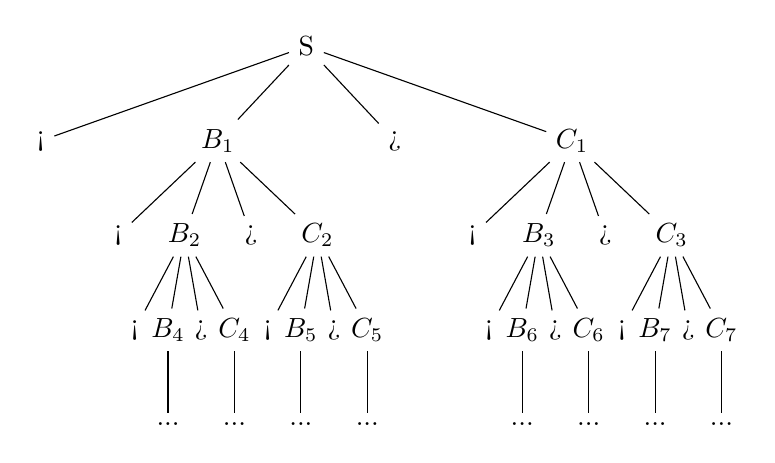
\begin{tikzpicture} [
  level 1/.style={sibling distance=8em},
  level 2/.style={sibling distance=3em},
  level 3/.style={sibling distance=1.5em},
  level 4/.style={sibling distance=1em},
	scale=0.8]
\node{S}
 child {node {<}}
 child {node {$B_1$}
      child {node {<}}
      child { node {$B_2$}
        child { node {<}}
        child { node {$B_4$}
        child {node {...}} }
        child {node {>}}
        child {node {$C_4$} child {node {...}} } }
      child {node {>}}
      child {node {$C_2$}
              child { node {<}}
              child { node {$B_5$}
                      child {node {...}} }
              child {node {>}}
             child {node {$C_5$} child {node {...}} } } }
 child {node {>}}
 child {node {$C_1$}
       child { node {<}}
       child { node {$B_3$}
             child { node {<}}
             child { node {$B_6$}
child {node {...}} }
             child {node {>}}
            child {node {$C_6$}
                 child {node {...}} }  }
       child {node {>}}
       child {node {$C_3$}
              child { node {<}}
             child { node {$B_7$}
             child {node {...}} }
             child {node {>}}
            child {node {$C_7$}
    child {node {...}} } }
     };
\end{tikzpicture}
 \\
	\caption{``Худшее`` дерево разбора для input-driven грамматики}
\label{IDw}
\end{figure}
По Лемме~\ref{Heightlem} в случае синтаксического анализа графа на $n$ вершинах высота данного дерева не превысит $|N|n^2$. Нетрудно заметить, что на каждом уровне дерева прибавляется в два раза больше листьев. По формуле суммы геометрической прогрессии получаем длину строки для данного дерева разбора:
\begin{equation}
\zeta \le 2^{|N|n^2 - 1} - 2
\end{equation}
\begin{corollaryrus}
Глубина схемы синтаксического разбора графа $D$ вершинах для случая input-driven грамматики $G$ равна $O(|N|n^2)$ для входа длиной $n$.
\end{corollaryrus}


\subsection{Оценка глубины схемы для LL(k) грамматик}
Пусть дана контекстно-свободная грамматика $G = (N, \Sigma, P, S)$. Рассмотрим два произвольных левосторонних вывода слова $w$ в этой грамматике:
\begin{itemize}
	\item $S \Rightarrow^* pA\beta \Rightarrow p \alpha \beta \Rightarrow^* py \eta$
	\item $S \Rightarrow^* pA\beta \Rightarrow p \alpha' \beta \Rightarrow^* py \xi$
\end{itemize}
где $p$ и $y$~--- цепочки из терминалов, уже разобранная часть слова $w$, $A$~--- нетерминал грамматики, в которой есть правила $A \rightarrow \alpha$ и $A \rightarrow \alpha'$, причем $\alpha, \alpha', \beta, \eta, \xi$~--- последовательности из терминалов и нетерминалов. Если из выполнения условий, что $|y| = k$ или $|y| < k$, $\eta = \xi = \varepsilon$, cледует равенство $\alpha = \alpha'$, то $G$ называется \textit{LL(k)-грамматикой}~\cite{LL}.

Практическое преимущество LL-грамматик состоит в том, что они позволяют \textit{синтаксический анализ сверху-вниз}~--- анализ, при котором анализатор исходит из предположения,что входная строка синтаксически верна, и, читая строку слева направо, обходит предполагаемое дерево разбора сверху вниз.

Оценим влияние величины параметра $k$ на структуру дерева разбора. По определению LL-грамматики, для каждого нетерминала и входной строки терминалов длиной $\le k$ должно существовать единственное правило вывода, которое однозначно определяется этой строкой и текущим нетерминалом при спуске сверху-вниз. Всего правил для одного нетерминала не более $\frac{\Sigma(\Sigma^{k-1} - 1)}{\Sigma -1}$. С точки зрения разбора графа, каждому нетерминалу должен соответствовать путь из $i$ в $j$. Тогда для каждого нетерминала должно существовать не менее одного уникального под пути длиной $\le k$. Таких подпутей может быть максимум $\frac{\Sigma(\Sigma^{k-1} - 1)}{\Sigma -1}$. Нас интересуют пути из $i$ в $j$ для каждого нетерминала, таких путей $n^2$. У $n^2$ путей должно быть как минимум $n$ начальных подпутей. Получаем $n \le \frac{\Sigma(\Sigma^{k-1} - 1)}{\Sigma -1}$ для каждого нетерминала. Пусть $k = 1$, тогда $n < \Sigma$, такую грамматику и граф можно подобрать, тогда в его дереве разбора будут существовать все тройки. Для $k>1$ подбор ещё легче сделать, так как правая часть неравенства растёт со скоростью геометрической прогрессии. 

Определение накладывает большие ограничения на грамматику. В частности, нельзя использовать левую рекурсию: если она есть, то анализатор зациклится, будет наращивать в стеке периодическую последовательность. Нормальный вид Грейбах, в котором все правила имеют вид $A \rightarrow a \alpha$, где $a \in \Sigma$ и $\alpha \in (\Sigma \cup N)^*$, не только исключает возможность левой рекурсии, но и вообще удобен для обработки строки слева направо. Пусть грамматика находится в квадратичной нормальной форме Грейбах. Грамматика находится в \textit{квадратичной нормальной форме Грейбах} тогда и только тогда, когда она в нормальной форме Грейбах и в правой части каждого правила не более двух нетерминалов. Розенкранц в работе~\cite{QuadGreib} доказал, что любая контекстно-свободная грамматика может быть представлена в квадратичной нормальной форме Грейбах. Поэтому построим ``худшее дерево`` для LL-грамматики в этой форме (рис.~\ref{LLw}). Предположим, что у нас соблюдаются выше описанные условия на соотношение $\Sigma$ и $n$.
\begin{figure}[h!]
\centering
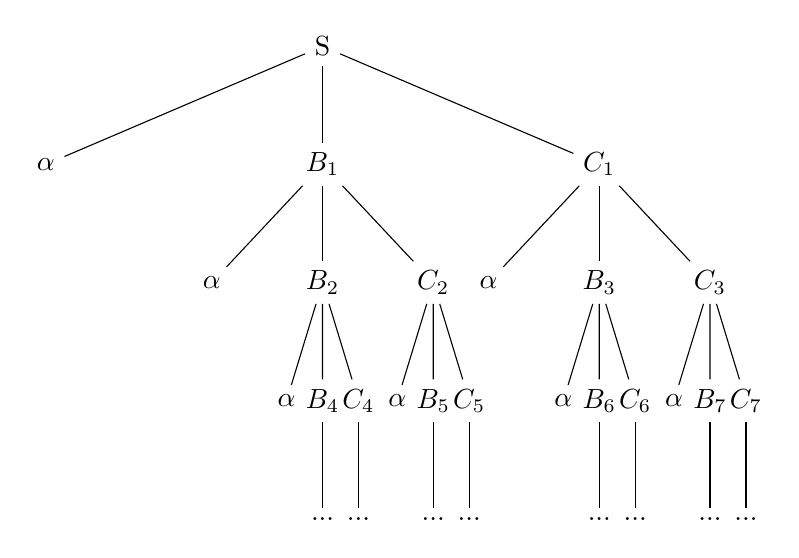
\begin{tikzpicture} [
  level 1/.style={sibling distance=10em},
  level 2/.style={sibling distance=4em},
  level 3/.style={sibling distance=1.3em},
  level 4/.style={sibling distance=0.05em}]
\node{S}
 child {node {$\alpha$}}
 child {node {$B_1$}
      child {node {$\alpha$}}
      child { node {$B_2$}
        child { node {$\alpha$}}
        child { node {$B_4$}
        child {node {...}} }
        child {node {$C_4$} child {node {...}} } }
      child {node {$C_2$}
              child { node {$\alpha$}}
              child { node {$B_5$}
                      child {node {...}} }
             child {node {$C_5$} child {node {...}} } } }
 child {node {$C_1$}
       child { node {$\alpha$}}
       child { node {$B_3$}
             child { node {$\alpha$}}
             child { node {$B_6$}
child {node {...}} }
            child {node {$C_6$}
                 child {node {...}} } }
       child {node {$C_3$}
              child { node {$\alpha$}}
             child { node {$B_7$}
             child {node {...}} }
            child {node {$C_7$}
    child {node {...}} } }
     };
\end{tikzpicture}
 \\
	\caption{``Худшее`` дерево разбора для грамматики в квадратичной нормальной форме Грейбах}
\label{LLw}
\end{figure}
Так как высота дерева не превышает $|N|n^2$, а количество листьев на каждом уровне растет со скоростью геометрической прогрессии со знаменателем 2, получаем:
\begin{equation}
\zeta \le 2^{|N|n^2 - 1} - 1
\end{equation}
\begin{corollaryrus}
Глубина схемы синтаксического разбора графа $D$ для случая LL(k) грамматики $G$ равна $O(|N|n^2)$ для входа длиной $n$.
\end{corollaryrus}
% У заключения нет номера главы
\section*{Заключение}
В рамках данной работы был предложен алгоритм синтаксического анализа ациклических графов. Благодаря топологической сортировке, которая задает порядок на вершинах графа, становится возможным использовать классические алгоритмы синтаксического анализа, использующие стратегию динамического программирования. Таким образом, на ациклических графах задачу можно решить за время умножения булевых матриц, как и обычную задачу синтаксического анализа на строках. Более того, предложенный алгоритм работает не только с контекстно-свободными грамматиками, но и с их расширением~--- булевыми грамматиками, что позволяет формировать более сложные запросы к графам.

Также была построена булева схема для решения задачи и дан адгоритм, обобщающий данную схему для модели SIMDAG. В общем случае, задача не может быть эффективно решена с помощью параллельной схемы, так как глубина схемы полиномиальна ($O(|N|n^2)$) от входа размером $n$ для произвольной контекстно-свободной грамматики. Но было показано, что глубина схемы зависит от максимальной длины строки, являющейся ответом на задачу. Данный показатель может быть полиномиальным от количества вершин в графе $D$, что даст эффективную схему логарифмической глубины. В работе показано, что к таким классам относятся линейный грамматики и языки Дика на одном типе скобок. Также данный показатель линеен от количества вершин в графе, в случае, если входной граф является ациклическим, поэтому для таких графов булева схема будет работать эффективно и иметь также полилогарифмическую глубину. К классам грамматик с максимальной строкой экспоненциального размера относятся input-driven грамматики и LL-грамматики, поэтому глубина схемы для них остается полиномиальной от размера входа.


\begin{thebibliography}{10}
\def\selectlanguageifdefined#1{
\expandafter\ifx\csname date#1\endcsname\relax
\else\selectlanguage{#1}\fi}
\providecommand*{\href}[2]{{\small #2}}
\providecommand*{\url}[1]{{\small #1}}
\providecommand*{\BibUrl}[1]{\url{#1}}
\providecommand{\BibAnnote}[1]{}
\providecommand*{\BibEmph}[1]{#1}
\ProvideTextCommandDefault{\cyrdash}{\iflanguage{russian}{\hbox
  to.8em{--\hss--}}{\textemdash}}
\providecommand*{\BibDash}{\ifdim\lastskip>0pt\unskip\nobreak\hskip.2em plus
  0.1em\fi
\cyrdash\hskip.2em plus 0.1em\ignorespaces}
\renewcommand{\newblock}{\ignorespaces}

\bibitem{IDGrammar}
\selectlanguageifdefined{english}
\BibEmph{Alur~Rajeev, Madhusudan~P.}
  \href{http://dx.doi.org/10.1145/1007352.1007390}{Visibly Pushdown
  Languages}~// Proceedings of the Thirty-sixth Annual ACM Symposium on Theory
  of Computing. \BibDash
\newblock STOC '04. \BibDash
\newblock New York, NY, USA~: ACM, 2004. \BibDash
\newblock P.~202--211.

\bibitem{MatrixMult}
\selectlanguageifdefined{english}
\BibEmph{Azimov~Rustam, Grigorev~Semyon}. Graph Parsing by Matrix
  Multiplication~// Proceedings of the 1st ACM SIGMOD Joint International Workshop on Graph Data Management Experiences \& Systems (GRADES) and Network Data Analytics (NDA). \BibDash
\newblock GRADES-NDA '18 \BibDash
\newblock New York, NY, USA~: ACM, 2018.
\newblock P.~5:1--5:10.

\bibitem{ConjPath}
\selectlanguageifdefined{english}
\BibEmph{Azimov~Rustam, Grigorev~Semyon}. Path querying using conjunctive
  grammars~//
  \href{http://dx.doi.org/10.15514/ISPRAS-2018-30(2)-8}{\BibEmph{Proceedings of
  the Institute for System Programming of the RAS}}. \BibDash
\newblock 2018. \BibDash 01. \BibDash
\newblock Vol.~30. \BibDash
\newblock P.~149--166.

\bibitem{GraphDB}
\selectlanguageifdefined{english}
\BibEmph{Barceló~Baeza~Pablo}. Querying graph databases~//
  \href{http://dx.doi.org/10.1145/2463664.2465216}{\BibEmph{Proceedings of the
  ACM SIGACT-SIGMOD-SIGART Symposium on Principles of Database Systems}}.
  \BibDash
\newblock 2013. \BibDash 06.

\bibitem{Bradford}
\selectlanguageifdefined{english}
\BibEmph{Bradford~Phillip~G.} Efficient Exact Paths For Dyck and semi-Dyck
  Labeled Path Reachability~// \BibEmph{CoRR}. \BibDash
\newblock 2018. \BibDash
\newblock Vol. abs/1802.05239. \BibDash
\newblock 1802.05239.

\bibitem{Brent}
\selectlanguageifdefined{english}
\BibEmph{Brent~Richard, M.~GOLDSCHLAGER~LESLIE}. A PARALLEL ALGORITHM FOR
  CONTEXT-FREE PARSING. \BibDash
\newblock 1983. \BibDash 01.

\bibitem{social}
\selectlanguageifdefined{english}
\BibEmph{Chaudhary~Anoop, FAISAL~ABDUL}. Role of graph databases in social
  networks. \BibDash
\newblock 2016. \BibDash 06.

\bibitem{Lohrey}
\selectlanguageifdefined{english}
Circuits and Expressions over Finite Semirings~/ Moses~Ganardi, Danny~Hucke,
  Daniel~König, Markus~Lohrey~//
  \href{http://dx.doi.org/10.1145/3241375}{\BibEmph{ACM Transactions on
  Computation Theory}}. \BibDash
\newblock 2018. \BibDash 08. \BibDash
\newblock Vol.~10. \BibDash
\newblock P.~1--30.

\bibitem{RDF}
\selectlanguageifdefined{english}
Context-Free Path Queries on {RDF} Graphs~/ Xiaowang~Zhang, Zhiyong~Feng,
  Xin~Wang, Guozheng~Rao~// \BibEmph{CoRR}. \BibDash
\newblock 2015. \BibDash
\newblock Vol. abs/1506.00743. \BibDash
\newblock 1506.00743.

\bibitem{Dyck1}
\selectlanguageifdefined{english}
\BibEmph{Deleage~Jean-Luc, Pierre~Laurent}. The rational index of the Dyck
  language $D_1$~//
  \href{http://dx.doi.org/10.1016/0304-3975(86)90158-1}{\BibEmph{Theoretical
  Computer Science}}. \BibDash
\newblock 1986. \BibDash
\newblock Vol.~47. \BibDash
\newblock P.~335 -- 343.

\bibitem{Dymond}
\selectlanguageifdefined{english}
\BibEmph{Dymond~Patrick~W.} Input-driven languages are in log n depth~//
  \href{http://dx.doi.org/10.1016/0020-0190(88)90148-2}{\BibEmph{Information
  Processing Letters}}. \BibDash
\newblock 1988. \BibDash
\newblock Vol.~26, no.~5. \BibDash
\newblock P.~247 -- 250.

\bibitem{Earley}
\selectlanguageifdefined{english}
\BibEmph{Earley~Jay}. An Efficient Context-free Parsing Algorithm~//
  \href{http://dx.doi.org/10.1145/362007.362035}{\BibEmph{Commun. ACM}}.
  \BibDash
\newblock 1970. \BibDash Feb. \BibDash
\newblock Vol.~13, no.~2. \BibDash
\newblock P.~94--102.

\bibitem{PCompl}
\selectlanguageifdefined{english}
\BibEmph{Greenlaw~Raymond, Hoover~H.~James, Ruzzo~Walter~L.} Limits to Parallel
  Computation: P-completeness Theory. \BibDash
\newblock New York, NY, USA~: Oxford University Press, Inc., 1995. \BibDash
\newblock
  ISBN:~\href{http://isbndb.com/search-all.html?kw=0-19-508591-4}{0-19-508591-4}.

\bibitem{Ibarra}
\selectlanguageifdefined{english}
\BibEmph{H.~Ibarra~Oscar, Jiang~Tao, Ravikumar~Bala}. Some Subclasses of
  Context-Free Languages In NC1.~//
  \href{http://dx.doi.org/10.1016/0020-0190(88)90047-6}{\BibEmph{Inf. Process.
  Lett.}} \BibDash
\newblock 1988. \BibDash 10. \BibDash
\newblock Vol.~29. \BibDash
\newblock P.~111--117.

\bibitem{HellConj}
\selectlanguageifdefined{english}
\BibEmph{Hellings~Jelle}. Conjunctive Context-Free Path Queries~// ICDT.
  \BibDash
\newblock 2014.

\bibitem{HellingsCFPQ}
\selectlanguageifdefined{english}
\BibEmph{Hellings~Jelle}. Path Results for Context-free Grammar Queries on
  Graphs~// \BibEmph{CoRR}. \BibDash
\newblock 2015. \BibDash
\newblock Vol. abs/1502.02242. \BibDash
\newblock 1502.02242.

\bibitem{LLComp}
\selectlanguageifdefined{english}
\BibEmph{Holzer~Markus, Lange~Klaus~J{\"o}rn}. On the complexities of linear
  LL(1) and LR(1) grammars~// Fundamentals of Computation Theory~/ Ed.\ by\
  Zolt{\'a}n~{\'E}sik. \BibDash
\newblock Berlin, Heidelberg~: Springer Berlin Heidelberg, 1993. \BibDash
\newblock P.~299--308.

\bibitem{Kasami}
\selectlanguageifdefined{english}
\BibEmph{Kasami~Tadao}. AN EFFICIENT RECOGNITION AND SYNTAX ANALYSIS ALGORITHM
  FOR CONTEXT-FREE LANGUAGES. \BibDash
\newblock 1965. \BibDash 07. \BibDash
\newblock P.~40.

\bibitem{Kelemenova}
\selectlanguageifdefined{english}
\BibEmph{Kelemenová~Alica}. Complexity of normal form grammars~//
  \href{http://dx.doi.org/10.1016/0304-3975(83)90026-9}{\BibEmph{Theoretical
  Computer Science}}. \BibDash
\newblock 1983. \BibDash
\newblock Vol.~28, no.~3. \BibDash
\newblock P.~299 -- 314.

\bibitem{LReach}
\selectlanguageifdefined{english}
\BibEmph{Komarath~Balagopal, Sarma~Jayalal, Sunil~K.~S.} On the Complexity of
  L-reachability~// \BibEmph{CoRR}. \BibDash
\newblock 2017. \BibDash
\newblock Vol. abs/1701.03255. \BibDash
\newblock \href{http://arxiv.org/abs/1701.03255}{1701.03255}.

\bibitem{Reg2}
\selectlanguageifdefined{english}
\BibEmph{Koschmieder~Andr{\'e}, Leser~Ulf}.
  \href{http://dx.doi.org/10.1007/978-3-642-31235-9_12}{Regular Path Queries on
  Large Graphs}~// Proceedings of the 24th International Conference on
  Scientific and Statistical Database Management. \BibDash
\newblock SSDBM'12. \BibDash
\newblock Berlin, Heidelberg~: Springer-Verlag, 2012. \BibDash
\newblock P.~177--194.

\bibitem{Reg1}
\selectlanguageifdefined{english}
\BibEmph{Mendelzon~Alberto~O., Wood~Peter~T.} Finding Regular Simple Paths in
  Graph Databases~//
  \href{http://dx.doi.org/10.1137/S009753979122370X}{\BibEmph{SIAM J. Comput.}}
  \BibDash
\newblock 1995. \BibDash Dec. \BibDash
\newblock Vol.~24, no.~6. \BibDash
\newblock P.~1235--1258.

\bibitem{boolean}
\selectlanguageifdefined{english}
\BibEmph{Okhotin~Alexander}. Boolean grammars~//
  \href{http://dx.doi.org/10.1016/j.ic.2004.03.006}{\BibEmph{Information and
  Computation}}. \BibDash
\newblock 2004. \BibDash
\newblock Vol. 194, no.~1. \BibDash
\newblock P.~19 -- 48.

\bibitem{OkhotinParse}
\selectlanguageifdefined{english}
\BibEmph{Okhotin~Alexander}. Parsing by matrix multiplication generalized to
  Boolean grammars~//
  \href{http://dx.doi.org/10.1016/j.tcs.2013.09.011}{\BibEmph{Theoretical
  Computer Science}}. \BibDash
\newblock 2014. \BibDash
\newblock Vol. 516. \BibDash
\newblock P.~101 -- 120.

\bibitem{conjunctive}
\selectlanguageifdefined{english}
\BibEmph{Okhotin~Alexander}.
  \href{http://dx.doi.org/10.1007/978-3-319-98654-8_4}{A Tale of Conjunctive
  Grammars: 22nd International Conference, DLT 2018, Tokyo, Japan, September
  10-14, 2018, Proceedings}. \BibDash
\newblock 2018. \BibDash 01. \BibDash
\newblock P.~36--59. \BibDash
\newblock
  ISBN:~\href{http://isbndb.com/search-all.html?kw=978-3-319-98653-1}{978-3-319-98653-1}.

\bibitem{OkhotinIDPDA}
\selectlanguageifdefined{english}
\BibEmph{Okhotin~Alexander, Salomaa~Kai}. Complexity of Input-driven Pushdown
  Automata~// \href{http://dx.doi.org/10.1145/2636805.2636821}{\BibEmph{SIGACT
  News}}. \BibDash
\newblock 2014. \BibDash Jun. \BibDash
\newblock Vol.~45, no.~2. \BibDash
\newblock P.~47--67.

\bibitem{CFRat}
\selectlanguageifdefined{english}
\BibEmph{Pierre~Laurent}. Rational indexes of generators of the cone of
  context-free languages~//
  \href{http://dx.doi.org/10.1016/0304-3975(92)90269-L}{\BibEmph{Theoretical
  Computer Science}}. \BibDash
\newblock 1992. \BibDash
\newblock Vol.~95, no.~2. \BibDash
\newblock P.~279 -- 305.

\bibitem{GreibRat}
\selectlanguageifdefined{en}
\BibEmph{Pierre~Laurent, Farinone~Jean-Marc}. Context-free languages with
  rational index in $\Theta (n^\gamma )$ for algebraic numbers $\gamma $~//
  \BibEmph{RAIRO - Theoretical Informatics and Applications - Informatique
  Th\'eorique et Applications}. \BibDash
\newblock 1990. \BibDash
\newblock Vol.~24, no.~3. \BibDash
\newblock P.~275--322.

\bibitem{Bio}
\selectlanguageifdefined{english}
Quantifying variances in comparative RNA secondary structure prediction~/
  James~WJ~Anderson, {\'A}d{\'a}m~Nov{\'a}k, Zsuzsanna~S{\"u}k{\"o}sd et~al.~//
  \href{http://dx.doi.org/10.1186/1471-2105-14-149}{\BibEmph{BMC
  Bioinformatics}}. \BibDash
\newblock 2013. \BibDash May. \BibDash
\newblock Vol.~14, no.~1. \BibDash
\newblock P.~149.

\bibitem{Reps}
\selectlanguageifdefined{english}
\BibEmph{Reps~Thomas}. Program Analysis via Graph Reachability~// Proceedings
  of the 1997 International Symposium on Logic Programming. \BibDash
\newblock ILPS '97. \BibDash
\newblock Cambridge, MA, USA~: MIT Press, 1997. \BibDash
\newblock P.~5--19.

\bibitem{Reg3}
\selectlanguageifdefined{english}
\BibEmph{Reutter~Juan~L., Romero~Miguel, Vardi~Moshe~Y.} Regular Queries on
  Graph Databases~//
  \href{http://dx.doi.org/10.1007/s00224-016-9676-2}{\BibEmph{Theor. Comp.
  Sys.}} \BibDash
\newblock 2017. \BibDash Jul. \BibDash
\newblock Vol.~61, no.~1. \BibDash
\newblock P.~31--83.

\bibitem{QuadGreib}
\selectlanguageifdefined{english}
\BibEmph{Rosenkrantz~Daniel}. Matrix Equations and Normal Forms for
  Context-Free Grammars~//
  \href{http://dx.doi.org/10.1145/321406.321412}{\BibEmph{J. ACM}}. \BibDash
\newblock 1967. \BibDash 07. \BibDash
\newblock Vol.~14. \BibDash
\newblock P.~501--507.

\bibitem{LL}
\selectlanguageifdefined{english}
\BibEmph{Rosenkrantz~D.J., Stearns~R.E.} Properties of deterministic top-down
  grammars~//
  \href{http://dx.doi.org/10.1016/S0019-9958(70)90446-8}{\BibEmph{Information
  and Control}}. \BibDash
\newblock 1970. \BibDash
\newblock Vol.~17, no.~3. \BibDash
\newblock P.~226 -- 256.

\bibitem{Regularrealizability}
\selectlanguageifdefined{english}
\BibEmph{Rubtsov~Alexander~A., Vyalyi~Mikhail~N.} Regular realizability
  problems and context-free languages~// \BibEmph{CoRR}. \BibDash
\newblock 2015. \BibDash
\newblock Vol. abs/1503.00295. \BibDash
\newblock 1503.00295.

\bibitem{Ruzzo}
\selectlanguageifdefined{english}
\BibEmph{Ruzzo~Walter~L.} On uniform circuit complexity~//
  \href{http://dx.doi.org/10.1016/0022-0000(81)90038-6}{\BibEmph{Journal of
  Computer and System Sciences}}. \BibDash
\newblock 1981. \BibDash
\newblock Vol.~22, no.~3. \BibDash
\newblock P.~365 -- 383.

\bibitem{Rytter}
\selectlanguageifdefined{english}
\BibEmph{Rytter~Wojciech}. On the recognition of context-free languages~//
  Computation Theory~/ Ed.\ by\ Andrzej~Skowron. \BibDash
\newblock Berlin, Heidelberg~: Springer Berlin Heidelberg, 1985. \BibDash
\newblock P.~318--325.

\bibitem{Swernofsky2015OnTC}
\selectlanguageifdefined{english}
\BibEmph{Swernofsky~Joseph, Wehar~Michael}. On the Complexity of Intersecting
  Regular, Context-Free, and Tree Languages~// ICALP. \BibDash
\newblock 2015.

\bibitem{Tarjan}
\selectlanguageifdefined{english}
\BibEmph{{Tarjan}~R.} \href{http://dx.doi.org/10.1109/SWAT.1971.10}{Depth-first
  search and linear graph algorithms}~// 12th Annual Symposium on Switching and
  Automata Theory (swat 1971). \BibDash
\newblock 1971. \BibDash Oct. \BibDash
\newblock P.~114--121.

\bibitem{Valiant}
\selectlanguageifdefined{english}
\BibEmph{Valiant~Leslie~G.} General context-free recognition in less than cubic
  time~//
  \href{http://dx.doi.org/10.1016/S0022-0000(75)80046-8}{\BibEmph{Journal of
  Computer and System Sciences}}. \BibDash
\newblock 1975. \BibDash
\newblock Vol.~10, no.~2. \BibDash
\newblock P.~308 -- 315.

\bibitem{Yonger}
\selectlanguageifdefined{english}
\BibEmph{Younger~Daniel~H.} Recognition and parsing of context-free languages
  in time n3~//
  \href{http://dx.doi.org/10.1016/S0019-9958(67)80007-X}{\BibEmph{Information
  and Control}}. \BibDash
\newblock 1967. \BibDash
\newblock Vol.~10, no.~2. \BibDash
\newblock P.~189 -- 208.

\bibitem{DyckTrees}
\selectlanguageifdefined{english}
\BibEmph{Yuan~Hao, Eugster~Patrick}. An Efficient Algorithm for Solving the
  Dyck-CFL Reachability Problem on Trees~// Programming Languages and Systems~/
  Ed.\ by\ Giuseppe~Castagna. \BibDash
\newblock Berlin, Heidelberg~: Springer Berlin Heidelberg, 2009. \BibDash
\newblock P.~175--189.

\bibitem{Static}
\selectlanguageifdefined{english}
\BibEmph{Zhang~Qirun, Su~Zhendong}. Context-sensitive Data-dependence Analysis
  via Linear Conjunctive Language Reachability~//
  \href{http://dx.doi.org/10.1145/3093333.3009848}{\BibEmph{SIGPLAN Not.}}
  \BibDash
\newblock 2017. \BibDash Jan. \BibDash
\newblock Vol.~52, no.~1. \BibDash
\newblock P.~344--358.

\bibitem{Warcha2012UsingNG}
\selectlanguageifdefined{english}
\BibEmph{Łukasz Warchał}. Using Neo4j graph database in social network
  analysis. \BibDash
\newblock 2012.

\bibitem{UlmanCompilers}
\selectlanguageifdefined{russian}
Компиляторы: принципы, технологии и
  инструментарий~/ Д.~Ульман, Р.~Сети, М.~Лам,
  А.~Ахо. \BibDash
\newblock ЛитРес, 2018. \BibDash
\newblock
  ISBN:~\href{http://isbndb.com/search-all.html?kw=9785041399252}{9785041399252}.

\bibitem{Hopcroft}
\selectlanguageifdefined{russian}
\BibEmph{Хопкрофт~Д.~Мотвани~Р.~Ульман~Д.}
  Введение в теорию автоматов, языков и
  вычислений, 2-е издание. \BibDash
\newblock Издательский дом Вильямс. \BibDash
\newblock
  ISBN:~\href{http://isbndb.com/search-all.html?kw=9785845902610}{9785845902610}.

\end{thebibliography}

